\documentclass{article}
\usepackage{tikz, amsmath, amssymb, pgfplots, enumerate}
\usetikzlibrary{shapes,arrows,calc}
\usepgfplotslibrary{fillbetween}
\usepackage[margin=1in]{geometry}

\title{Consumer Theory Concepts}
\author{Ryan Safner}
\date{ECON 306}

\begin{document}

\maketitle

\section*{Consumer's Constrained Optimization}

\begin{itemize}
	\item \textbf{Constrained optimization} (in general) always involves the following three elements: 
	\begin{enumerate}
		\item \textbf{Choose:} \textcolor{blue}{$<$some alternative$>$}
		\item \textbf{In order to maximize:} \textcolor{green}{$<$some objective$>$}
		\item \textbf{Subject to}: \textcolor{red}{$<$some constraints$>$}
	\end{enumerate}
	\item The \textbf{Consumer's (constrained optimization) problem} is:  
	\begin{enumerate}
		\item \textbf{Choose:} \textcolor{blue}{$<$bundle of goods$>$}
		\item \textbf{In order to maximize:} \textcolor{green}{$<$utility$>$}
		\item \textbf{Subject to}: \textcolor{red}{$<$income and market prices$>$}
	\end{enumerate}

\end{itemize}

\subsection*{Choices}
\begin{itemize}
	\item Consumers choose bundles of goods:
	\begin{equation*}
	(x,y)	
	\end{equation*}
	where $x$ = amount of good $x$, and $y$ = amount of good $y$
\end{itemize}

\subsection*{Constraints: The Budget Constraint}

\begin{itemize}
	\item \textbf{Budget set}: the set of all bundles of goods that are \emph{affordable}: 
	\begin{equation*}
	p_x x+p_y y \leq m 	
	\end{equation*}
	\begin{itemize}
		\item Consumers can buy bundles that do not spend all income (income leftover)  
	\end{itemize}
	\item \textbf{Budget constraint}: the set of all bundles of goods that \emph{spend all income} 
	\begin{equation*}
	p_x x+p_y y = m 	
	\end{equation*}
	\begin{itemize}
		\item To graph, solve for $y$: 
		\begin{equation*}
			y=\frac{m}{p_y}-\frac{p_x}{p_y}x 
		\end{equation*}
		\clearpage 
		\begin{itemize}
		\item Vertical intercept: $\displaystyle \frac{m}{p_y}$
		\item Horizontal intercept: $\displaystyle \frac{m}{p_x}$
		\item Slope: $\displaystyle -\frac{p_x}{p_y}$
		\end{itemize}
	\end{itemize} 
	\begin{figure}[h!]
		\centering 
			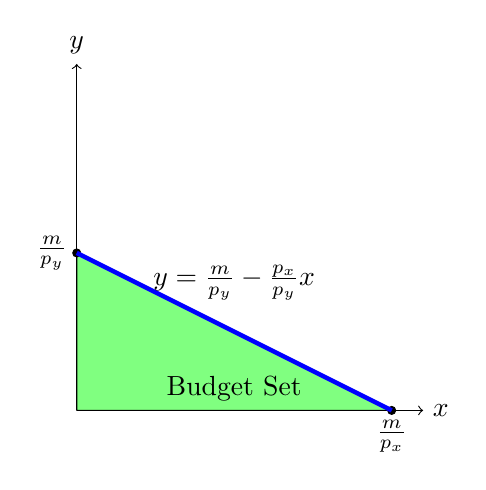
\begin{tikzpicture}[scale=.4]
			\draw[fill=green!50](0,0)--(0,5)--(10,0)--node[above]{\textcolor{black}{Budget Set}}(0,0);
			\draw[->] (0,0) -- (11,0) coordinate (x axis) node[right]{$x$};
 			\draw[->] (0,0) -- (0,11) coordinate (y axis) node[above]{$y$};
 			\draw[black, fill=black] (0,5)circle(0.125cm)node[left]{$\frac{m}{p_y}$};
 			\draw[black, fill=black] (10,0)circle(0.125cm)node[below]{$\frac{m}{p_x}$};
			\draw[ultra thick, blue] (0,5)--node[above=.25cm]{\textcolor{black}{$y=\frac{m}{p_y}-\frac{p_x}{p_y}x$}}(10,0);
 		\end{tikzpicture}
	\caption{The Budget Constraint (blue) and Budget Set (green)}
	\end{figure} 
	\item All points on the line spend all income
	\begin{itemize}
		\item All points beneath line are \emph{affordable} (in budget set) but do not spend all income
		\item All points above the line are \emph{not} affordable at current income and prices 	
	\end{itemize}

	\item Budget constraint determined by three parameters: $p_x, p_y, m$
	\begin{itemize}
		\item Change in income: shifts budget constraint in parallel 
		\begin{itemize}
			\item New $m'$ in intercepts 
			\item No change in slope 
		\end{itemize}
		\item Change in a market price: rotates budget constraint 
		\begin{itemize}
			\item New intercept for good that changed in price
			\item New slope 
		\end{itemize}
	\end{itemize} 
	\item Slope of budget constraint measures the \emph{market} exchange rate between $x$ and $y$ (their relative prices)
\end{itemize}

\begin{table}[h!]
		\centering 
		\begin{tabular}{ccc}
$\Delta m$ ($\uparrow$ in green, $\downarrow$ in red) & $\Delta p_x$ ($\uparrow$ in red, $\downarrow$ in green) & $\Delta p_y$ ($\uparrow$ in red, $\downarrow$ in green)\\
			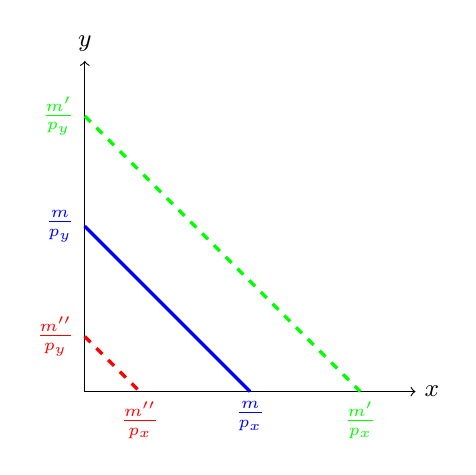
\begin{tikzpicture}[scale=0.7]\small 
			\draw[->] (0,0) -- (6,0) coordinate (x axis) node[right]{$x$};
 			\draw[->] (0,0) -- (0,6) coordinate (y axis) node[above]{$y$};
	\draw[very thick, blue] (0,3)node[left]{$\frac{m}{p_y}$}--(3,0)node[below]{$\frac{m}{p_x}$};
	\draw[very thick, green, dashed] (0,5)node[left]{$\frac{m'}{p_y}$}--(5,0)node[below]{$\frac{m'}{p_x}$};
	\draw[very thick, red, dashed] (0,1)node[left]{$\frac{m''}{p_y}$}--(1,0)node[below]{$\frac{m''}{p_x}$};
\end{tikzpicture}
&
	\begin{tikzpicture}[scale=0.7]\small 
			\draw[->] (0,0) -- (6,0) coordinate (x axis) node[right]{$x$};
 			\draw[->] (0,0) -- (0,6) coordinate (y axis) node[above]{$y$};
	\draw[very thick, blue] (0,3)node[left]{$\frac{m}{p_y}$}--(3,0)node[below]{$\frac{m}{p_x}$};
	\draw[very thick, red, dashed] (0,3)--(1,0)node[below]{$\frac{m}{p_x'}$};
	\draw[very thick, green, dashed] (0,3)--(5,0)node[below]{$\frac{m}{p_x''}$};
\end{tikzpicture}
&
	\begin{tikzpicture}[scale=0.7]\small 
			\draw[->] (0,0) -- (6,0) coordinate (x axis) node[right]{$x$};
 			\draw[->] (0,0) -- (0,6) coordinate (y axis) node[above]{$y$};
	\draw[very thick, blue] (0,3)node[left]{$\frac{m}{p_y}$}--(3,0)node[below]{$\frac{m}{p_x}$};
	\draw[very thick, red, dashed] (0,1)node[left]{$\frac{m}{p_y'}$}--(3,0);
	\draw[very thick, green, dashed] (0,5)node[left]{$\frac{m}{p_y''}$}--(3,0);
\end{tikzpicture}\\
\end{tabular}
\caption{How the budget constraint changes with income and market prices} 
\end{table}

\clearpage 

\subsection*{Objective: Utility and Preferences}
\begin{itemize}
	\item \textbf{Preferences} express rankings between bundles of goods
	\begin{itemize}
		\item For any two bundles of goods $a$ and $b$: 
		\begin{itemize}
			\item $a \succ b$: $a$ is preferred to $b$
			\item $a \prec b$: $b$ is preferred to $a$
			\item $a \sim b$: indifferent between $a$ and $b$
	\end{itemize}
	\item Assumptions about ``well-behaved'' preferences: 
	\begin{enumerate}
		\item Reflexivity: $a \succeq a$
		\item Completeness: for all $a$ and $b$: $a \succ b$, $a \prec b$, or $a \sim b$
		\item Transitivity: if $a \succ b$ and $b \succ c \implies a \succ c$
		\end{enumerate} 
	\end{itemize}
	\item \textbf{Indifference curves} link all bundles which the consumer is indifferent between 
							\begin{figure}[h!]
							\centering 
	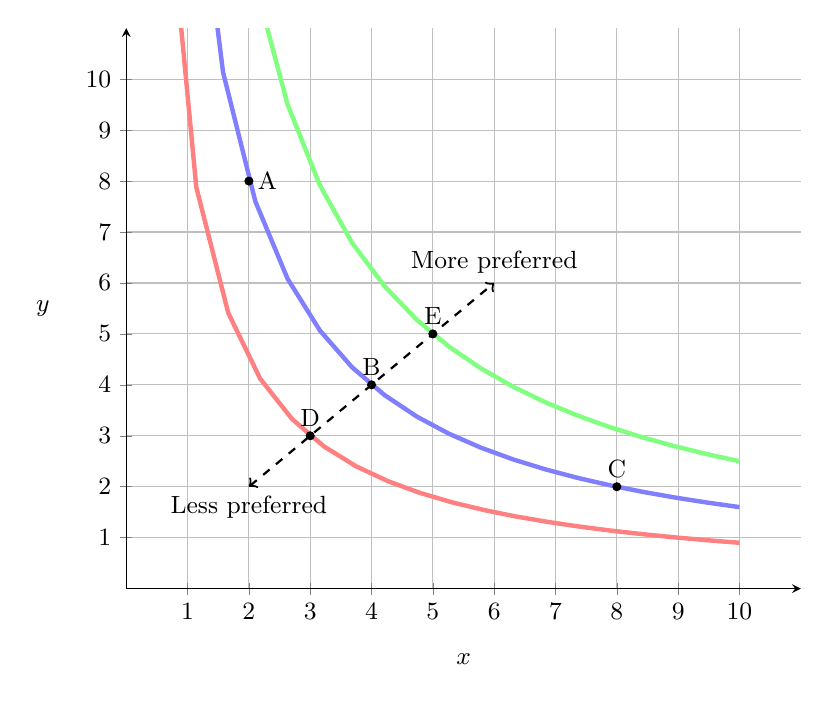
\begin{tikzpicture}\small  
	\begin{axis}[
		scale=1.25,
		axis lines=middle, 
		enlarge x limits={rel=0.1, upper},
		enlarge y limits={rel=0.1, upper},
		every axis x label/.style={at={(axis description cs:0.5,-0.1)},anchor=north},
		every axis y label/.style={at={(axis description cs:-0.1,0.5)},anchor=east},
	%legend pos=outer north east,
	xlabel=$x$,
	ylabel=$y$,
	shader=flat,
	xtick={1, 2,...,10},
	ytick={0,1,2,...,10},
	grid=major,
	ymin=0,
	xmin=0,
	xmax=10,
	ymax=10,
]
	\addplot[name path=ic, domain=0:10, samples=20, ultra thick, color=blue!50]{16/(x)};
	\draw[black, fill=black] (axis cs:2,8)circle(0.05cm)node[right]{A};
	\draw[black, fill=black] (axis cs:8,2)circle(0.05cm)node[above]{C};
	\draw[black, fill=black] (axis cs:4,4)circle(0.05cm)node[above]{B};
	\addplot[domain=0.1:10, samples=20, ultra thick, color=red!50]{9/(x)};
	\draw[black, fill=black] (axis cs:3,3)circle(0.05cm)node[above]{D};
	\addplot[domain=0:10, samples=20, ultra thick, color=green!50]{25/(x)};
	\draw[black, fill=black] (axis cs:5,5)circle(0.05cm)node[above]{E};
	\draw[thick, black, dashed, <->] (axis cs:2,2)node[below]{Less preferred}--(axis cs:6,6)node[above]{More preferred};
\end{axis}
\end{tikzpicture}
\caption{Indifference curves: $E \succ A \sim B \sim C \succ D$}
\end{figure}
	\begin{itemize}
		\item Assumptions of ``well-behaved'' indifference curves: 
		\begin{enumerate}
			\item We can always draw indifference curves
			\item Monotonicity: ``more is preferred to less''
			\item Convexity: ``averages are preferred to extremes''
			\item Transitivity: indifference curves can never cross
		\end{enumerate}
		\clearpage
		\item In general, even non-monotonic indifference curves (i.e. when there is 1 or more \textbf{bads}) follow a pattern. Figure 3 shows four types of indifference curves, broken down into four quadrants. Black arrows show the direction of \emph{better} bundles in each of the four cases: 
		\begin{enumerate}[I.]
			\item $x$ is a good, $y$ is a bad
			\item $x$ and $y$ are both bads
			\item $x$ and $y$ are both goods
			\item $x$ is a bad, $y$ is a good 
		\end{enumerate}
	\begin{figure}[h!]
		\centering 	
			\begin{tikzpicture}\small 
	\begin{axis}[
		scale=1.5,
		axis lines=middle, 
		enlarge x limits={rel=0.1, upper},
		enlarge y limits={rel=0.1, upper},
		every axis y label/.style={at={(axis description cs:-0.1,0.5)},rotate=90,anchor=north},
		every axis x label/.style={at={(axis description cs:0.5,-0.1)},anchor=north},
	%legend pos=outer north east,
	xlabel=$x$,
	ylabel=$y$,
	shader=flat,
	ticks=none,
	grid=none,
	ymin=0,
	xmin=0,
	xmax=5,
	ymax=5,
]
	\addplot[opacity=0]{x};
	\draw[thick, blue!50] (axis cs: 2.5,2.5) circle[radius=100];
	\draw[thick, blue!75] (axis cs: 2.5,2.5) circle[radius=150];
	\draw[thick, blue] (axis cs: 2.5,2.5) circle[radius=200];
	\draw[ultra thick, dashed, red](axis cs:0,2.5)--(axis cs:5,2.5);
	\draw[ultra thick, dashed, red](axis cs:2.5,0)--(axis cs:2.5,5);
	\draw[thick, dashed, ->] (axis cs:1.25,1)--(axis cs: 2,2);
	\draw[thick, dashed, ->] (axis cs:1.25,4)--(axis cs: 2,3);
	\draw[thick, dashed, ->] (axis cs:3.75,1)--(axis cs: 3,2);
	\draw[thick, dashed, ->] (axis cs:3.75,4)--(axis cs: 3,3);
	\draw[red] (axis cs:1,4)node[above]{I};
	\draw[red] (axis cs:4,4)node[above]{II};
	\draw[red] (axis cs:1,1)node[below]{III};
	\draw[red] (axis cs:4,1)node[below]{IV};
\end{axis}
\end{tikzpicture}
\caption{Possible indifference curves with goods and bads. Arrows show direction of higher utility for each quadrant.}
	\end{figure}
	
	\item \textbf{Marginal rate of substitution (MRS)}: an individual's exchange rate between good $x$ and $y$
		\begin{itemize}
		\item $MRS=$ the slope of the indifference curve
		\item Literally: the amount of $y$ given up to obtain 1 more $x$ and remain indifferent 
		\end{itemize}
	\end{itemize}
	\item \textbf{Utility function}: represents preferences in functional form
	\begin{equation*}
	u(x,y)	
	\end{equation*}
	\begin{itemize}
		\item We can assign utility levels to any bundles such that for any bundles $a$ and $b$: 
		\begin{equation*}
		a \succ b \iff u(a) > u(b)	
		\end{equation*}
 		\item Utility is \textbf{ordinal} not \textbf{cardinal}!
 		\begin{itemize}
 			\item The actual utility numbers for bundle $a$ and $b$ mean nothing literally!
 			\item All that matters is if $u(a) > u(b)$, the consumer prefers $a$ over $b$ (we can't say \emph{how much})
 			\item Implies that multiple utility functions can represent the same preferences 
		\end{itemize}
		\item All points on the same indifference curve yield the same utility 
		\item \textbf{Marginal utility}: the change in utility from a 1-unit increase in consumption of a good 
		\begin{align*}
		MU_x&=\frac{\Delta u(x,y)}{\Delta x}\\
		MU_y&=\frac{\Delta u(x,y)}{\Delta y}\\	
		\end{align*}
 		\begin{itemize}
 			\item Marginal utilities are related to the MRS: 
 			\begin{equation*}
 			MRS=\frac{MU_x}{MU_y}	
 			\end{equation*}
 										\begin{figure}[h!]
							\centering 
	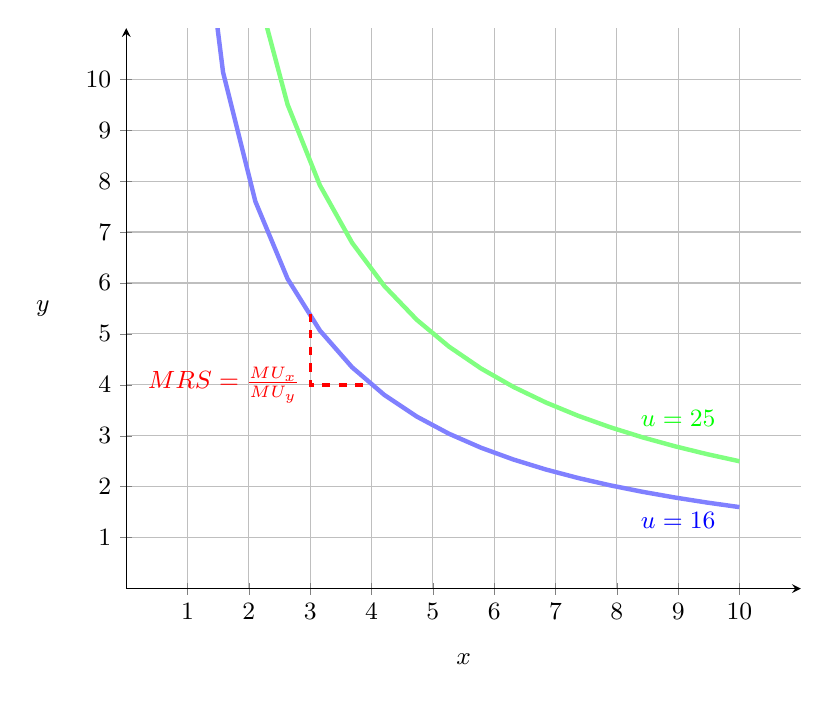
\begin{tikzpicture}\small  
	\begin{axis}[
		scale=1.25,
		axis lines=middle, 
		enlarge x limits={rel=0.1, upper},
		enlarge y limits={rel=0.1, upper},
		every axis x label/.style={at={(axis description cs:0.5,-0.1)},anchor=north},
		every axis y label/.style={at={(axis description cs:-0.1,0.5)},anchor=east},
	%legend pos=outer north east,
	xlabel=$x$,
	ylabel=$y$,
	shader=flat,
	xtick={1, 2,...,10},
	ytick={0,1,2,...,10},
	grid=major,
	ymin=0,
	xmin=0,
	xmax=10,
	ymax=10,
]
	\addplot[name path=ic, domain=0:10, samples=20, ultra thick, color=blue!50]{16/(x)};
	\draw[blue](axis cs:9,1)node[above]{$u=16$};
	\addplot[name path=ic, domain=0:10, samples=20, ultra thick, color=green!50]{25/(x)};
	\draw[green](axis cs:9,3)node[above]{$u=25$};
	\draw[very thick, dashed, red] (axis cs:3,5.4)--(axis cs:3,4)node[left]{$MRS=\frac{MU_x}{MU_y}$}--(axis cs:4,4);
\end{axis}
\end{tikzpicture}
\caption{Indifference curves for $u(x,y)=xy$}
\end{figure}
	\end{itemize}
	
	\clearpage 
	
	\item Shape \& slopes (MRS) of indifference curves:
	\begin{itemize}
		\item Steep vs. flat $\implies$ relative intensity of preference for $x$ vs. $y$  
	\begin{table}[h!]
		\centering 
		\begin{tabular}{cc}
			Vertical $\implies$ $y$ is a neutral (more$\sim$less $y$) & Horizontal $\implies$ $x$ is a neutral (more$\sim$less $x$)\\
			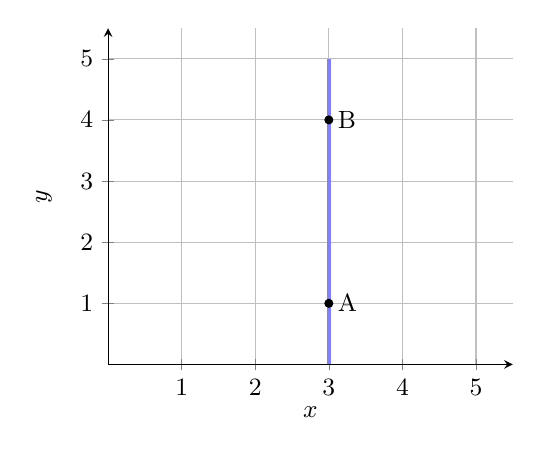
\begin{tikzpicture}\small 
	\begin{axis}[
		scale=0.75,
		axis lines=middle, 
		enlarge x limits={rel=0.1, upper},
		enlarge y limits={rel=0.1, upper},
		every axis y label/.style={at={(axis description cs:-0.2,0.5)},rotate=90,anchor=north},
		every axis x label/.style={at={(axis description cs:0.5,-0.1)},anchor=north},
	%legend pos=outer north east,
	xlabel=$x$,
	ylabel=$y$,
	shader=flat,
	xtick={1, 2,...,5},
	ytick={0,1,...,5},
	grid=major,
	ymin=0,
	xmin=0,
]
	\addplot[opacity=0]{x};
	\draw[very thick, blue!50](axis cs: 3,0)--(axis cs:3,5);
	\draw[fill=black](axis cs:3,1)circle(0.05cm)node[right]{A};
	\draw[fill=black](axis cs:3,4)circle(0.05cm)node[right]{B};
\end{axis}
\end{tikzpicture}
&
	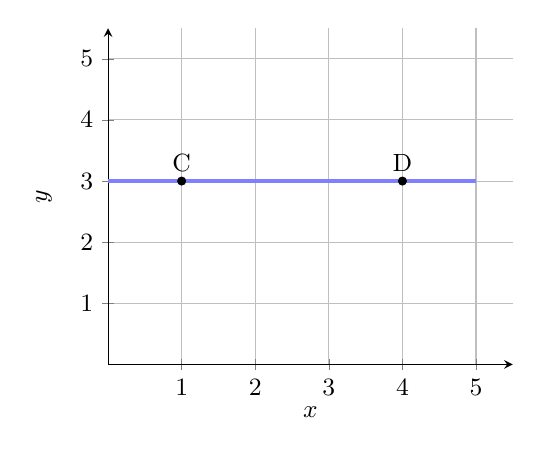
\begin{tikzpicture}\small 
	\begin{axis}[
		scale=0.75,
		axis lines=middle, 
		enlarge x limits={rel=0.1, upper},
		enlarge y limits={rel=0.1, upper},
		every axis y label/.style={at={(axis description cs:-0.2,0.5)},rotate=90,anchor=north},
		every axis x label/.style={at={(axis description cs:0.5,-0.1)},anchor=north},
	%legend pos=outer north east,
	xlabel=$x$,
	ylabel=$y$,
	xtick={1, 2,...,5},
	ytick={0,1,...,5},
	grid=major,
	ymin=0,
	xmin=0,
]
	\addplot[opacity=0]{x};
	\draw[very thick, blue!50](axis cs: 0,3)--(axis cs:5,3);
	\draw[fill=black](axis cs:1,3)circle(0.05cm)node[above]{C};
	\draw[fill=black](axis cs:4,3)circle(0.05cm)node[above]{D};
\end{axis}
\end{tikzpicture}\\
& \\ 
Steeper $\implies$ willing to give up more $y$ for $x$ & Flatter $\implies$ willing to give up less $y$ for $x$  \\
 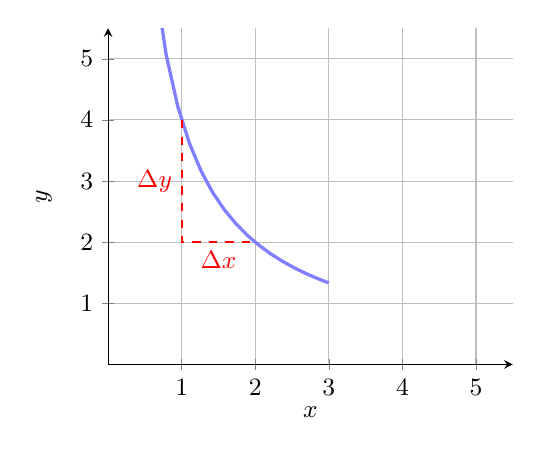
\begin{tikzpicture}\small 
	\begin{axis}[
		scale=0.75,
		axis lines=middle, 
		enlarge x limits={rel=0.1, upper},
		enlarge y limits={rel=0.1, upper},
		every axis y label/.style={at={(axis description cs:-0.2,0.5)},rotate=90,anchor=north},
		every axis x label/.style={at={(axis description cs:0.5,-0.1)},anchor=north},
	%legend pos=outer north east,
	xlabel=$x$,
	ylabel=$y$,
	xtick={1, 2,...,5},
	ytick={0,1,...,5},
	grid=major,
	ymin=0,
	xmin=0,
	ymax=5,
	xmax=5
]
	\addplot[very thick, blue!50, domain=0:3, samples=20]{4/(x)};
	\draw[thick, red, dashed] (axis cs:1,4)--node[left]{$\Delta y$}(axis cs:1,2)--node[below]{$\Delta x$}(axis cs:2,2);
\end{axis}
\end{tikzpicture}
&
			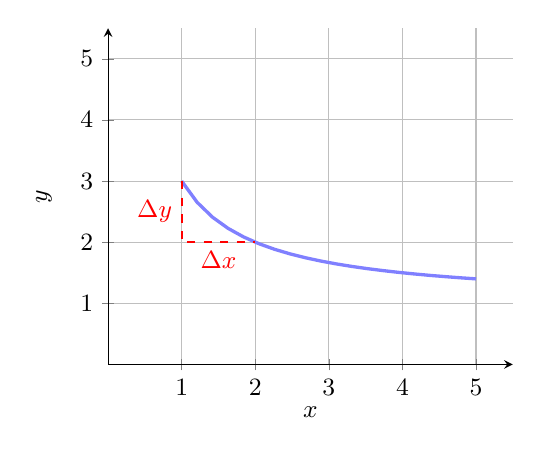
\begin{tikzpicture}\small 
	\begin{axis}[
		scale=0.75,
		axis lines=middle, 
		enlarge x limits={rel=0.1, upper},
		enlarge y limits={rel=0.1, upper},
		every axis y label/.style={at={(axis description cs:-0.2,0.5)},rotate=90,anchor=north},
		every axis x label/.style={at={(axis description cs:0.5,-0.1)},anchor=north},
	%legend pos=outer north east,
	xlabel=$x$,
	ylabel=$y$,
	shader=flat,
	xtick={1, 2,...,5},
	ytick={0,1,...,5},
	grid=major,
	ymin=0,
	xmin=0,
	ymax=5,
	xmax=5
]
	\addplot[very thick, blue!50, domain=1:5, samples=20]{2/x+1};
	\draw[thick, red, dashed] (axis cs:1,3)--node[left]{$\Delta y$}(axis cs:1,2)--node[below]{$\Delta x$}(axis cs:2,2);
\end{axis}
\end{tikzpicture}\\
		\end{tabular}
	\end{table}
	\item Bent vs. straight $\implies$ complementarity vs. substitutability between $x$ and $y$
		\begin{table}[h!]
		\centering 
		\begin{tabular}{cc}
			Right-angle $\implies$ perfect complements & Straight line $\implies$ perfect substitutes\\
			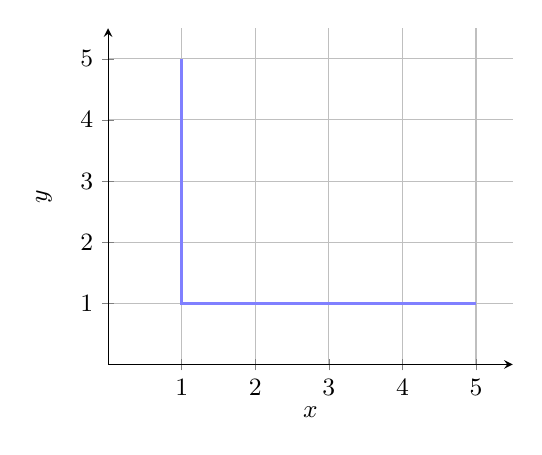
\begin{tikzpicture}\small 
	\begin{axis}[
		scale=0.75,
		axis lines=middle, 
		enlarge x limits={rel=0.1, upper},
		enlarge y limits={rel=0.1, upper},
		every axis y label/.style={at={(axis description cs:-0.2,0.5)},rotate=90,anchor=north},
		every axis x label/.style={at={(axis description cs:0.5,-0.1)},anchor=north},
	%legend pos=outer north east,
	xlabel=$x$,
	ylabel=$y$,
	shader=flat,
	xtick={1, 2,...,5},
	ytick={0,1,...,5},
	grid=major,
	ymin=0,
	xmin=0,
]
	\addplot[opacity=0]{x};
	\draw[very thick, blue!50] (axis cs:1,5)--(axis cs:1,1)--(axis cs:5,1);
\end{axis}
\end{tikzpicture}
&
	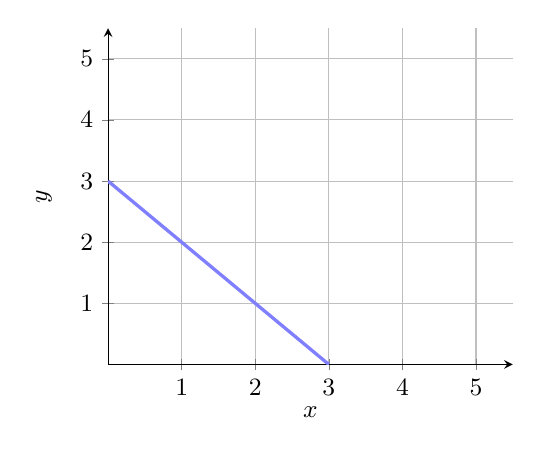
\begin{tikzpicture}\small 
	\begin{axis}[
		scale=0.75,
		axis lines=middle, 
		enlarge x limits={rel=0.1, upper},
		enlarge y limits={rel=0.1, upper},
		every axis y label/.style={at={(axis description cs:-0.2,0.5)},rotate=90,anchor=north},
		every axis x label/.style={at={(axis description cs:0.5,-0.1)},anchor=north},
	%legend pos=outer north east,
	xlabel=$x$,
	ylabel=$y$,
	xtick={1, 2,...,5},
	ytick={0,1,...,5},
	grid=major,
	ymin=0,
	xmin=0,
]
	\addplot[opacity=0]{x};
	\draw[very thick, blue!50] (axis cs:0,3)--(axis cs:3,0);
\end{axis}
\end{tikzpicture}\\
Always consume at same rate of combination & Always substitute at same rate\\
\end{tabular}
\end{table}
	\end{itemize}
\end{itemize}
	\clearpage 

\subsection*{Solving the Consumer's Problem}

\begin{itemize}
	\item Consumer chooses bundle of $x$ and $y$ to maximize utility subject to their income and market prices 	
	\begin{itemize}
		\item Expressed mathematically: 
	\begin{equation*}
		\max_{\textcolor{blue}{x,y}} \textcolor{green}{u(x,y)	}
		\end{equation*}
		\begin{equation*}
		\text{ s. t. }\textcolor{red}{p_xx+p_yy=m} 
	\end{equation*}
		\item Graphically: optimum is the point of tangency between the highest indifference curve and the budget constraint
				\begin{figure}[h!]
		\centering 
			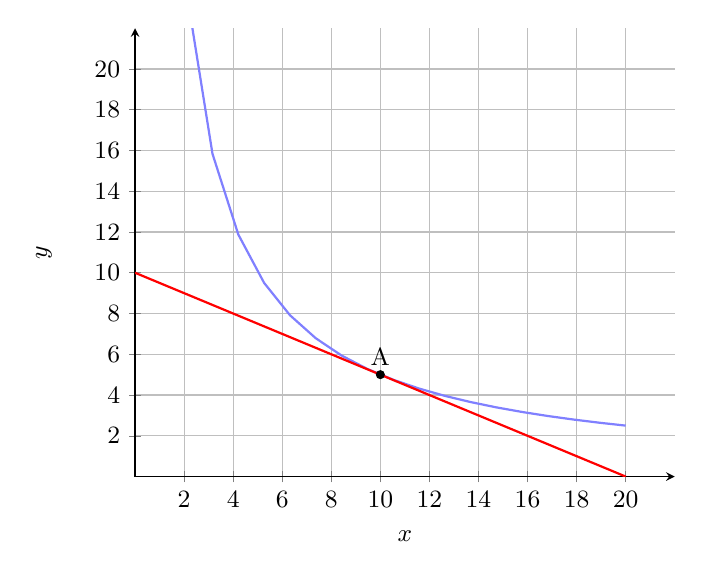
\begin{tikzpicture}\small  
	\begin{axis}[
		scale=1,
		axis lines=middle, 
		enlarge x limits={rel=0.1, upper},
		enlarge y limits={rel=0.1, upper},
		every axis y label/.style={at={(axis description cs:-0.2,0.5)},rotate=90,anchor=north},
		every axis x label/.style={at={(axis description cs:0.5,-0.1)},anchor=north},
	legend style={at={(0.5,-0.25)},anchor=north},
	ylabel=$y$,
	xlabel=$x$,
	xtick={2,4,...,20},
	ytick={0,2,...,20},
	grid=major,
	ymin=0,
	xmin=0,
	ymax=20,
	xmax=20
]
	\addplot[thick, color=blue!50, domain=0:20, samples=20, forget plot]{50/x};
	\draw[thick, red](axis cs:0,10)--(axis cs:20,0);
	\addlegendimage{thick, red};
	\addlegendimage{thick, blue!50};
	\draw[fill=black](axis cs:10,5)circle(0.05cm)node[above]{A};
\end{axis}
\end{tikzpicture}	
\caption{The consumer's optimum at point $A$: indifference curve is tangent to budget constraint}
		\end{figure}
		\item At the tangency point ($A$), all of the following are true: 
		\begin{align*}
		|\text{Slope of I.C.}|	&=|\text{Slope of B.C.}| & & \text{Slopes are equal}\\
		MRS&=\frac{p_x}{p_y} & & \text{Definition of each slope}\\
		\frac{MU_x}{MU_y}&=\frac{p_x}{p_y} & & \text{Individual exchange rate same as market exchange rate}\\
		\frac{MU_x}{p_x}&=\frac{MU_y}{p_y} & & \text{Marginal utility per \$1 is the same between $x$ and $y$}\\
		\end{align*}
		\end{itemize}
	\item \textbf{Equimarginal principle}: utility is optimized when individual can get no more utility by spending \$1 more on either $x$ or $y$
	\begin{itemize}
		\item Consumer is indifferent between buying more $x$ or buying more $y$: has no reason to change consumption decisions! 
		\item If marginal utility per dollar were greater for (e.g.) $x$ than for $y$, could buy more $x$ and get more utility! 
	\end{itemize}
	\end{itemize} 
\end{itemize}

\clearpage 
\section*{Deriving Demand}

\begin{itemize}
	\item An individual's \textbf{Demand (for good $x$)} is the optimal quantity that the individual would consume given current market prices and income: 
	\begin{equation*}
	q=D(p_x,p_y,m)
	\end{equation*}
	We explore how a person's demand changes as one of the parameters to the demand function changes: 
	\item Income effects $\bigg(\displaystyle \frac{\Delta q}{\Delta m} \bigg)$: how demand changes with income 
				\begin{table}[h!]
		\centering 
		\begin{tabular}{cc}
			Normal goods & Inferior good ($x$)\\
			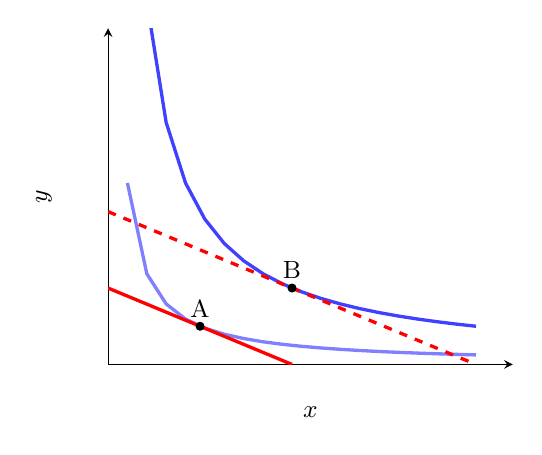
\begin{tikzpicture}\small 
	\begin{axis}[
		scale=0.75,
		axis lines=middle, 
		enlarge x limits={rel=0.1, upper},
		enlarge y limits={rel=0.1, upper},
		every axis y label/.style={at={(axis description cs:-0.2,0.5)},rotate=90,anchor=north},
		every axis x label/.style={at={(axis description cs:0.5,-0.1)},anchor=north},
	%legend pos=outer north east,
	xlabel=$x$,
	ylabel=$y$,
	shader=flat,
	ticks=none,
	grid=none,
	ymin=0,
	xmin=0,
	xmax=20,
	ymax=20,
]
	\addplot[opacity=0]{x};
	\addplot[very thick, color=blue!50, domain=0:20, samples=20, forget plot]{12.5/x};
	\addplot[very thick, color=blue!75, domain=0:20, samples=20, forget plot]{50/x};
	\draw[very thick, red](axis cs:0,5)--(axis cs:10,0);
	\draw[very thick, red, dashed](axis cs:0,10)--(axis cs:20,0);
	\draw[fill=black](axis cs:10,5)circle(0.05cm)node[above]{B};
	\draw[fill=black](axis cs:5,2.5)circle(0.05cm)node[above]{A};
\end{axis}
\end{tikzpicture}
&
	\begin{tikzpicture}\small 
	\begin{axis}[
		scale=0.75,
		axis lines=middle, 
		enlarge x limits={rel=0.1, upper},
		enlarge y limits={rel=0.1, upper},
		every axis y label/.style={at={(axis description cs:-0.2,0.5)},rotate=90,anchor=north},
		every axis x label/.style={at={(axis description cs:0.5,-0.1)},anchor=north},
	%legend pos=outer north east,
	xlabel=$x$,
	ylabel=$y$,
	ticks=none,
	grid=none,
	ymin=0,
	xmin=0,
	xmax=80,
	ymax=80,
]
	\addplot[domain=10:40, samples=25, very thick, color=blue!50]{200/(x)};
	\addplot[domain=5:40, samples=25, very thick, color=blue!75]{50/(x)+30};
	\draw[very thick, red] (axis cs:0,20)--(axis cs:40,0);
	\draw[very thick, dashed, red] (axis cs:0,40)--(axis cs:80,0);
	\draw[fill=black] (axis cs:20,10)circle(0.05cm)node[above]{A};
	\draw[fill=black] (axis cs:10,35)circle(0.05cm)node[above]{B};
\end{axis}
\end{tikzpicture}\\
Consume more $x$ and $y$ with $\uparrow$ m & Consume less $x$, more $y$ with $\uparrow$ m\\
\end{tabular}
\end{table}
	\begin{itemize}
		\item \textbf{Income Elasticity of Demand}: how responsive consumption is to changes in income 
		\begin{equation*}
		\epsilon_{q,m}=\frac{\% \Delta q}{\% \Delta m}=\cfrac{\bigg(\frac{(q_2-q_1)}{q_1}\bigg)}{\bigg(\frac{(m_2-m_1)}{m_1}\bigg)}
		\end{equation*}
		\begin{itemize}
			\item Measures the \% change in quantity consumed for a 1\% change in income
			\begin{itemize}
				\item i.e. ``if income changes by 1\%, quantity consumed changes by \emph{$\epsilon_{q,m}$}\%''
			\end{itemize}
			\item If $\epsilon>0$: \textbf{normal good}: consume more with higher income (and vice versa) 
			\begin{itemize}
				\item If $0 < \epsilon <1$: \textbf{necessity}: increase consumption by proportionately less than income increase 
				\item If $\epsilon >1$: \textbf{luxury}: increase consumption by proportionately more than income increase 
			\end{itemize}
			\item If $\epsilon<0$: \textbf{inferior good}: consume less with higher income (and vice versa) 
		\end{itemize}
	\end{itemize}
	\item Price effects $\bigg(\displaystyle \frac{\Delta q}{\Delta p} \bigg)$: how demand changes with price
	\begin{itemize}
		\item \textbf{Substitution effect}: change in consumption due to change in relative prices 
		\begin{itemize}
			\item Buy more of the relatively cheaper good, less of the relatively more expensive good
			\item Always the same direction, the primary reason for the law of demand (as $p \downarrow, q \uparrow$)
			\item Graphically: new bundle of $x$ and $y$ at \emph{new} exchange rate that yields \emph{same} utility as before
			\begin{itemize}
				\item Shift \emph{new} budget constraint inwards parallel until tangent to original indifference curve
				\item Movement from $A \rightarrow B$
			\end{itemize}
		\end{itemize}
		\item \textbf{Real Income effect}: change in consumption due to change in purchasing power
		\begin{itemize}
			\item A cheaper good frees up ability to buy more (less) goods overall (and vice versa), despite no change in \emph{nominal} income
			\item Positive for normal goods, negative for inferior goods! 
			\item Often smaller than the substitution effect
			\item Larger for goods that are a large portion of budget (e.g. housing, cars, etc) 
			\item Graphically: new bundle of $x$ and $y$ at new exchange rate that yields \emph{more} utility than before
			\begin{itemize}
				\item Movement from $B \rightarrow C$
			\end{itemize}
		\end{itemize}
		\item \textbf{Total price effect} $=$ substitution effect $+$ real income effect
		\begin{itemize}
			\item Graphically: overall movement from $A \rightarrow C$
			\item \textbf{Law of demand}: $\downarrow p, \uparrow q$
		\end{itemize}		
		\begin{table}[h!]
		\centering 
		\begin{tabular}{ccc}
$x$ is a Normal Good & $x$ is an Inferior Good & $x$ is a Giffen Good\\
		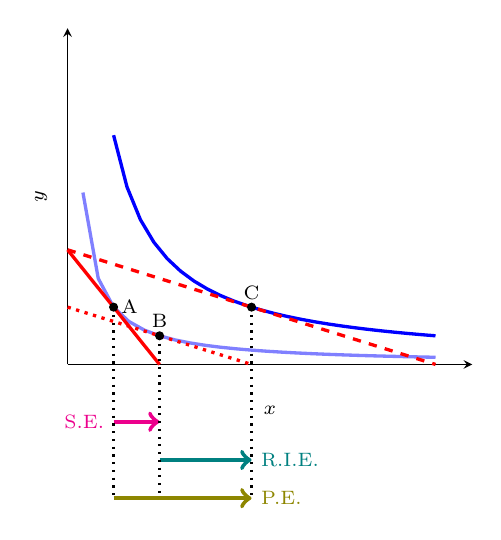
\begin{tikzpicture}\scriptsize 
	\begin{axis}[clip=false,
		scale=0.75,
		axis lines=middle, 
		enlarge x limits={rel=0.1, upper},
		enlarge y limits={rel=0.1, upper},
		every axis y label/.style={at={(axis description cs:-0.1,0.5)},rotate=90,anchor=north},
		every axis x label/.style={at={(axis description cs:0.5,-0.1)},anchor=north},
	%legend pos=outer north east,
	xlabel=$x$,
	ylabel=$y$,
	shader=flat,
	ticks=none,
	grid=none,
	ymin=0,
	xmin=0,
	ymax=80,
	xmax=80,
]
	\addplot[domain=0:80, samples=25, very thick, color=blue!50]{150/(x)};
	\addplot[domain=10:80, samples=25, very thick, color=blue]{600/(x)};
	\draw[very thick, red] (axis cs:0,30)--(axis cs:20,0);
	\draw[very thick, dashed, red] (axis cs:0,30)--(axis cs:80,0);
	\draw[very thick, dotted, red] (axis cs:0,15)--(axis cs:40,0);
	\draw[fill=black] (axis cs:10,15)circle(0.05cm)node[right]{A};
	\draw[fill=black] (axis cs:20,7.5)circle(0.05cm)node[above]{B};
	\draw[fill=black] (axis cs:40,15)circle(0.05cm)node[above]{C};
	\draw[->, ultra thick, magenta] (axis cs:10,-15)node[left]{S.E.}--(axis cs:20,-15);
	\draw[->, ultra thick, teal] (axis cs:20,-25)--(axis cs:40,-25)node[right]{R.I.E.};
	\draw[->,ultra thick, olive] (axis cs:10,-35)--(axis cs:40,-35)node[right]{P.E.};
	\draw[thick, dotted] (axis cs:10,15)--(axis cs:10,-35);
	\draw[thick, dotted] (axis cs:20,7.5)--(axis cs:20,-35);
	\draw[thick, dotted] (axis cs:40,15)--(axis cs:40,-35);
\end{axis}
\end{tikzpicture}
&
		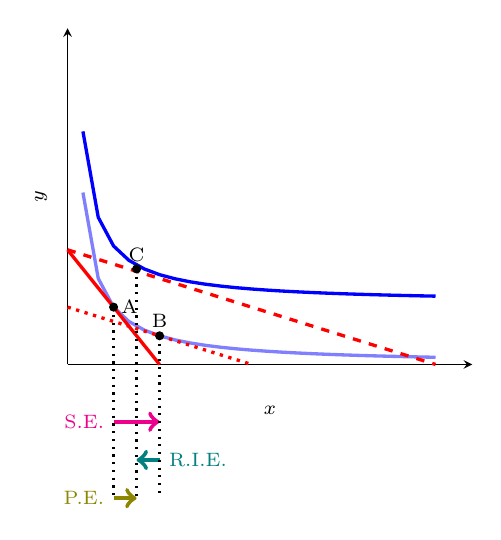
\begin{tikzpicture}\scriptsize 
	\begin{axis}[clip=false,
		scale=0.75,
		axis lines=middle, 
		enlarge x limits={rel=0.1, upper},
		enlarge y limits={rel=0.1, upper},
		every axis y label/.style={at={(axis description cs:-0.1,0.5)},rotate=90,anchor=north},
		every axis x label/.style={at={(axis description cs:0.5,-0.1)},anchor=north},
	%legend pos=outer north east,
	xlabel=$x$,
	ylabel=$y$,
	shader=flat,
	ticks=none,
	grid=none,
	ymin=0,
	xmin=0,
	ymax=80,
	xmax=80,
]
	\addplot[domain=0:80, samples=25, very thick, color=blue!50]{150/(x)};
	\addplot[domain=0:80, samples=25, very thick, color=blue]{150/(x)+16};
	\draw[very thick, red] (axis cs:0,30)--(axis cs:20,0);
	\draw[very thick, dashed, red] (axis cs:0,30)--(axis cs:80,0);
	\draw[very thick, dotted, red] (axis cs:0,15)--(axis cs:40,0);
	\draw[fill=black] (axis cs:10,15)circle(0.05cm)node[right]{A};
	\draw[fill=black] (axis cs:20,7.5)circle(0.05cm)node[above]{B};
	\draw[fill=black] (axis cs:15,25)circle(0.05cm)node[above]{C};
	\draw[->, ultra thick, magenta](axis cs:10,-15)node[left]{S.E.}--(axis cs:20,-15);
	\draw[->, ultra thick, teal] (axis cs:20,-25)node[right]{R.I.E.}--(axis cs:15,-25);
	\draw[->, ultra thick, olive] (axis cs:10,-35)node[left]{P.E.}--(axis cs:15,-35);
	\draw[thick, dotted] (axis cs:10,15)--(axis cs:10,-35);
	\draw[thick, dotted] (axis cs:20,7.5)--(axis cs:20,-35);
	\draw[thick, dotted] (axis cs:15,25)--(axis cs:15,-35);
\end{axis}
\end{tikzpicture}
&
		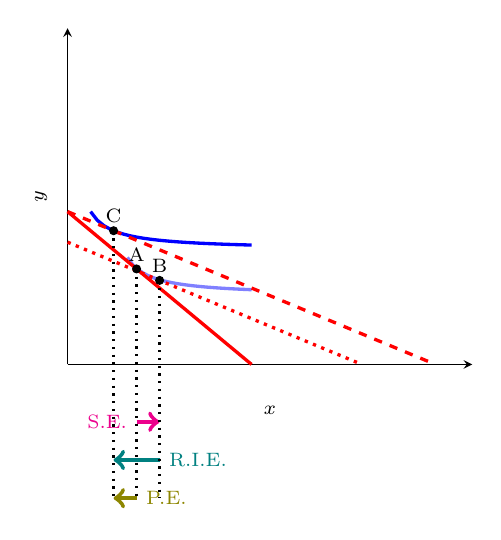
\begin{tikzpicture}\scriptsize 
	\begin{axis}[clip=false,
		scale=0.75,
		axis lines=middle, 
		enlarge x limits={rel=0.1, upper},
		enlarge y limits={rel=0.1, upper},
		every axis y label/.style={at={(axis description cs:-0.1,0.5)},rotate=90,anchor=north},
		every axis x label/.style={at={(axis description cs:0.5,-0.1)},anchor=north},
	%legend pos=outer north east,
	xlabel=$x$,
	ylabel=$y$,
	shader=flat,
	ticks=none,
	grid=none,
	ymin=0,
	xmin=0,
	ymax=80,
	xmax=80,
]
	\addplot[domain=5:40, samples=25, very thick, color=blue]{50/(x)+30};
	\addplot[domain=13:40, samples=25, very thick, color=blue!50]{50/(x-8)+18};
	\draw[very thick, red] (axis cs:0,40)--(axis cs:40,0);
	\draw[very thick, dashed, red] (axis cs:0,40)--(axis cs:80,0);
	\draw[very thick, dotted, red] (axis cs:0,32)--(axis cs:64,0);
	\draw[fill=black] (axis cs:15,25)circle(0.05cm)node[above]{A};
	\draw[fill=black] (axis cs:10,35)circle(0.05cm)node[above]{C};
	\draw[fill=black] (axis cs:20,22)circle(0.05cm)node[above]{B};
		\draw[->, ultra thick, magenta](axis cs:15,-15)node[left]{S.E.}--(axis cs:20,-15);
	\draw[->, ultra thick, teal] (axis cs:20,-25)node[right]{R.I.E.}--(axis cs:10,-25);
	\draw[->, ultra thick, olive] (axis cs:15,-35)node[right]{P.E.}--(axis cs:10,-35);
	\draw[thick, dotted] (axis cs:15,25)--(axis cs:15,-35);
	\draw[thick, dotted] (axis cs:20,22)--(axis cs:20,-35);
	\draw[thick, dotted] (axis cs:10,35)--(axis cs:10,-35);
\end{axis}
\end{tikzpicture}\\
\end{tabular}
\caption{\textcolor{magenta}{Substitution effects ($A \rightarrow B$)}, \textcolor{teal}{Real income effects ($B \rightarrow C$)}, and \textcolor{olive}{Price effects ($A \rightarrow C$)} for a decrease in the price of $x$} 
\end{table}
\item \textbf{Giffen good}: theoretical good that violates law of demand ($\downarrow p, \downarrow q$), requires:
		\begin{itemize}
			\item Negative real income effect (an inferior good)
			\item Real income effect $>$ substitution effect (good is a very very large portion of budget)
		\end{itemize} 
	\end{itemize}
	\item Cross-price effects $\bigg(\displaystyle \frac{\Delta q_x}{\Delta p_y} \bigg)$: how demand changes with price of \emph{other} goods
	\begin{itemize}
		\item \textbf{Cross-Price Elasticity of Demand}: how responsive consumption is to changes in price of \emph{another} good 
		\begin{equation*}
		\epsilon_{qx,py}=\frac{\% \Delta q_x}{\% \Delta p_y}=\cfrac{\bigg(\frac{(qx_2-q_1)}{qx_1}\bigg)}{\bigg(\frac{(py_2-py_1)}{py_1}\bigg)}
		\end{equation*}
		\begin{itemize}
			\item Measures the \% change in quantity consumed for a 1\% change in price of another good
			\begin{itemize}
				\item i.e. ``if price of $y$ changes by 1\%, quantity of $x$ consumed changes by \emph{$\epsilon_{qx,py}$}\%''
			\end{itemize}
			\item If $\epsilon>0$: $x$ and $y$ are \textbf{substitutes}: $\downarrow p_y, \downarrow q_x; \uparrow p_y, \uparrow q_x$
			\begin{itemize}
				\item e.g. Pepsi becoming cheaper reduces demand for Coke (switch to cheaper substitute) 
			\end{itemize} 
			\item If $\epsilon<0$: $x$ and $y$ are \textbf{complements}: $\downarrow p_y, \uparrow q_x; \uparrow p_y, \downarrow q_x$
						\begin{itemize}
				\item e.g. Milk becoming cheaper boosts demand for Cereal (the combination is now cheaper) 
			\end{itemize} 
		\end{itemize}
	\end{itemize} 
\end{itemize}

\end{document}
